\setcounter{chapter}{2}
\chapwithtoc{Appendix B: Minimal triangle dissections}

Figure \ref{fig:min-triangle-dissections} shows examples of minimal $\circledast$-free prime dissections for triangles of sizes up to 37. The full list is attached on the DVD.

\bigskip

\begin{figure}[htb]
\centering
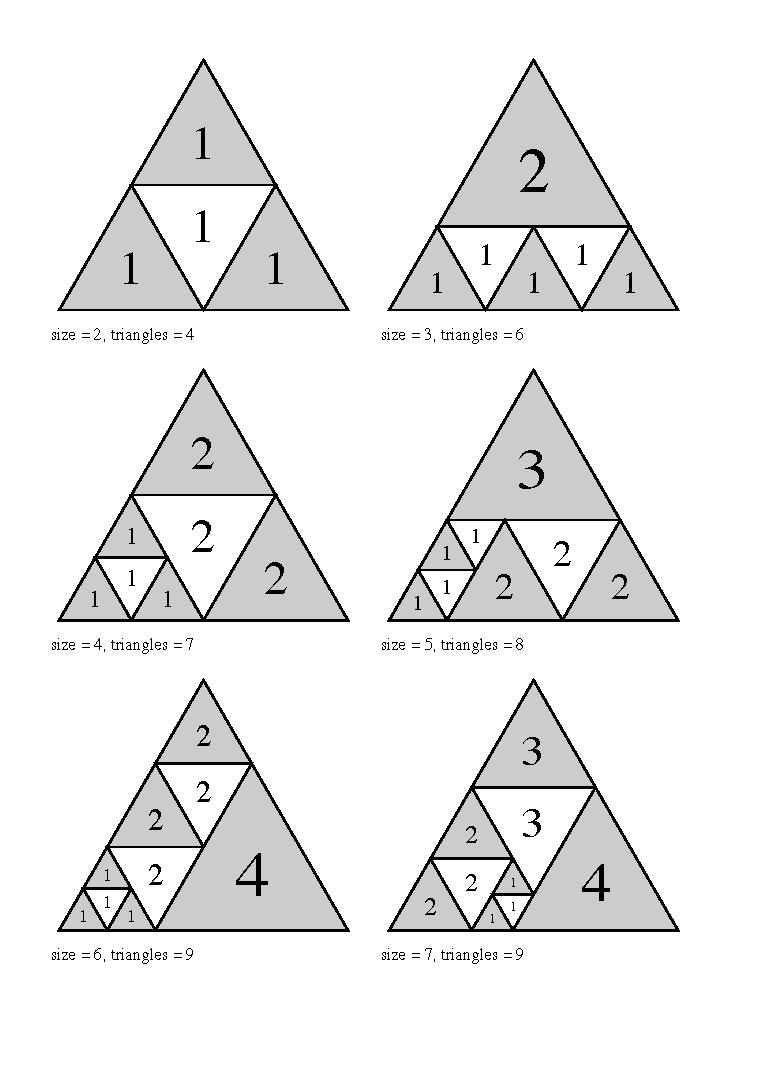
\includegraphics[trim=2em 4em 3em 2em, width=0.85\textwidth]{img/tranquility1.pdf}
\caption{Minimal triangle dissections.}
\label{fig:min-triangle-dissections}
\end{figure}

\begin{figure}[htb]
\centering
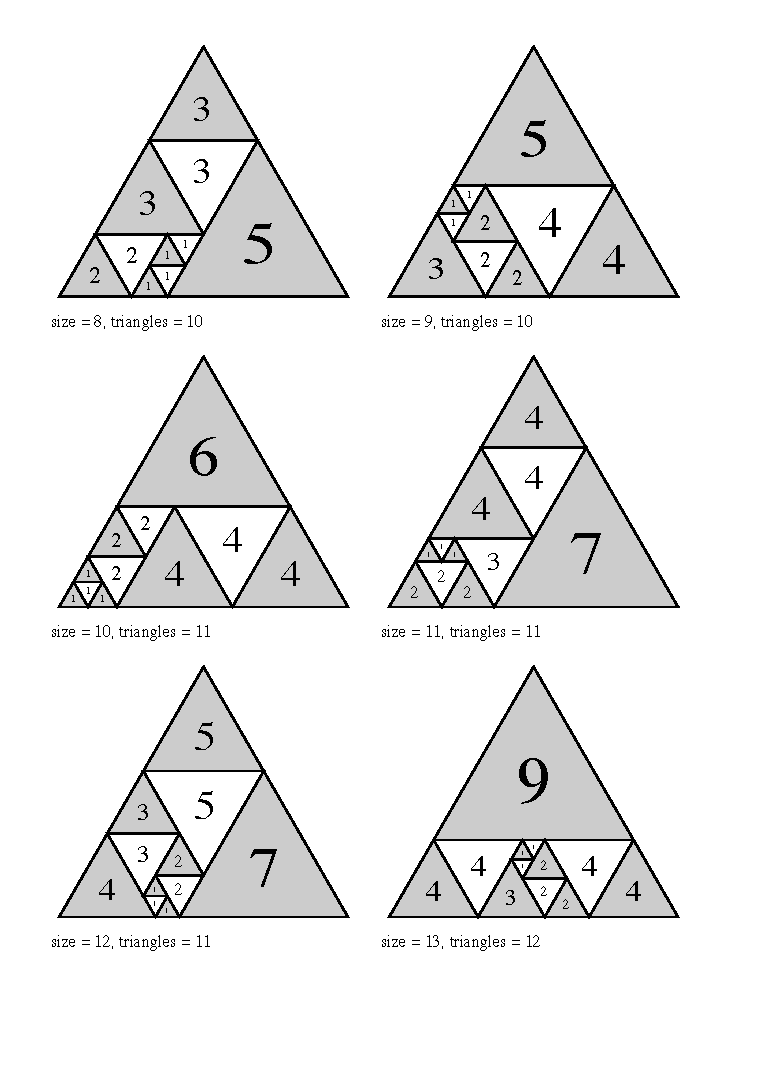
\includegraphics[trim=2em 4em 3em 2em, width=0.95\textwidth]{img/tranquility2.pdf}
\caption{Minimal triangle dissections.}
\end{figure}

\begin{figure}[htb]
\centering
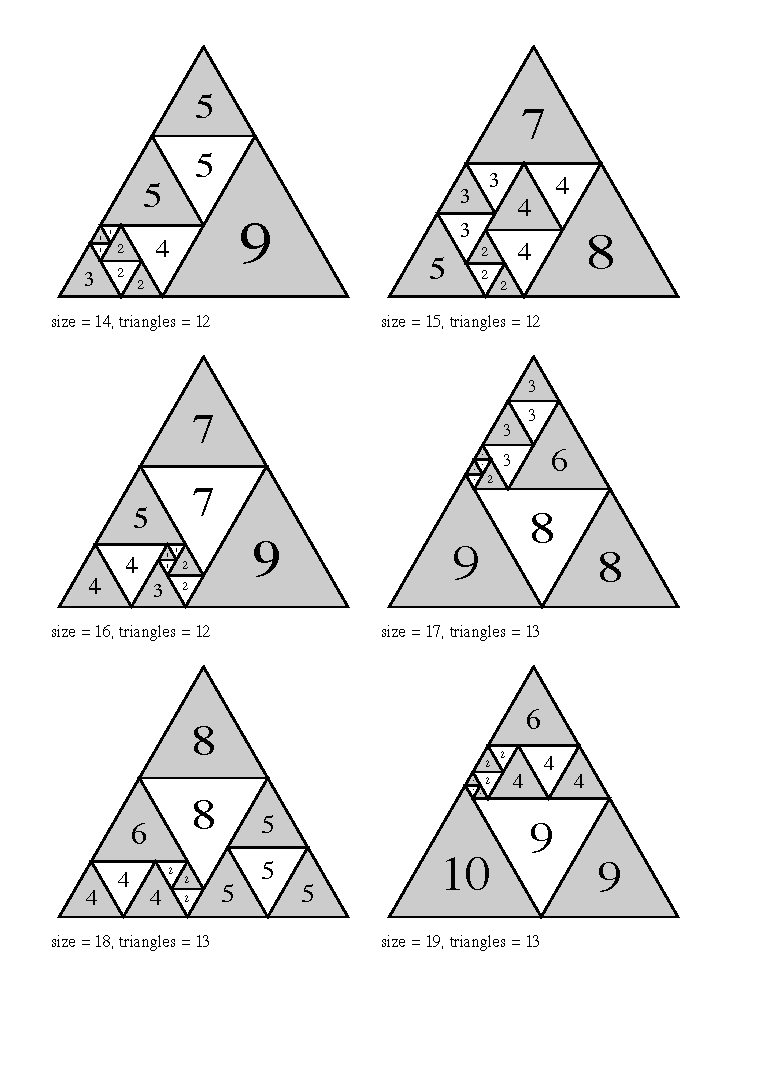
\includegraphics[trim=2em 4em 3em 2em, width=0.95\textwidth]{img/tranquility3.pdf}
\caption{Minimal triangle dissections.}
\end{figure}

\begin{figure}[htb]
\centering
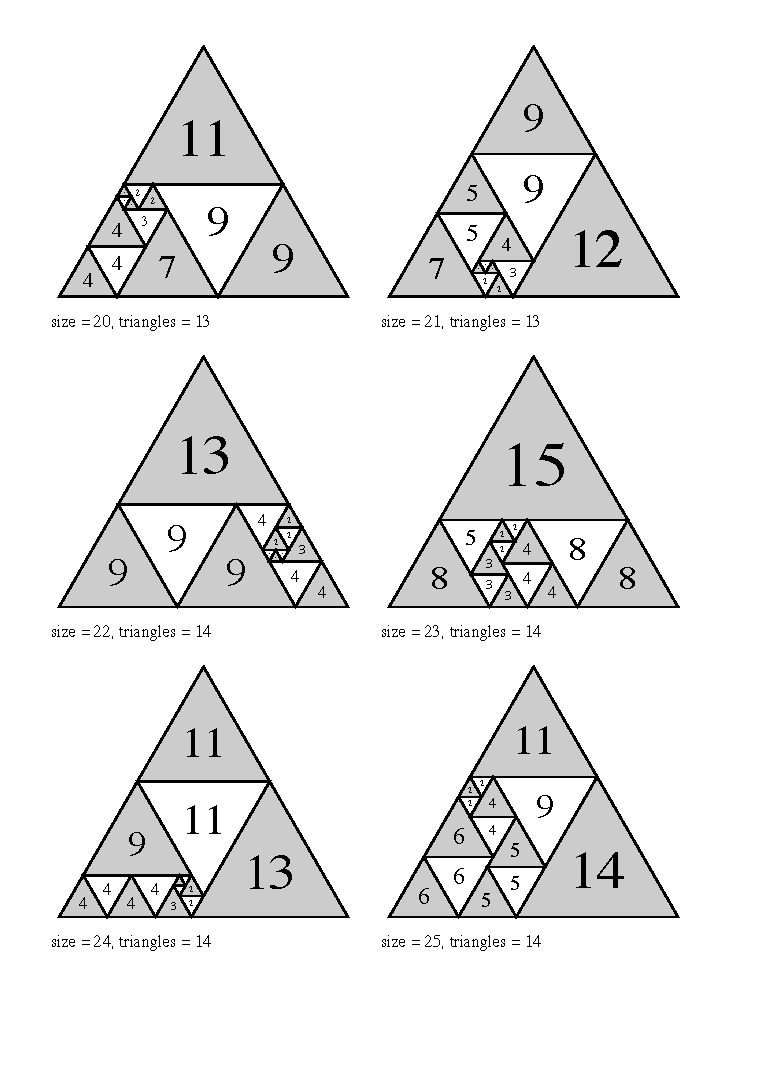
\includegraphics[trim=2em 4em 3em 2em, width=0.95\textwidth]{img/tranquility4.pdf}
\caption{Minimal triangle dissections.}
\end{figure}

\begin{figure}[htb]
\centering
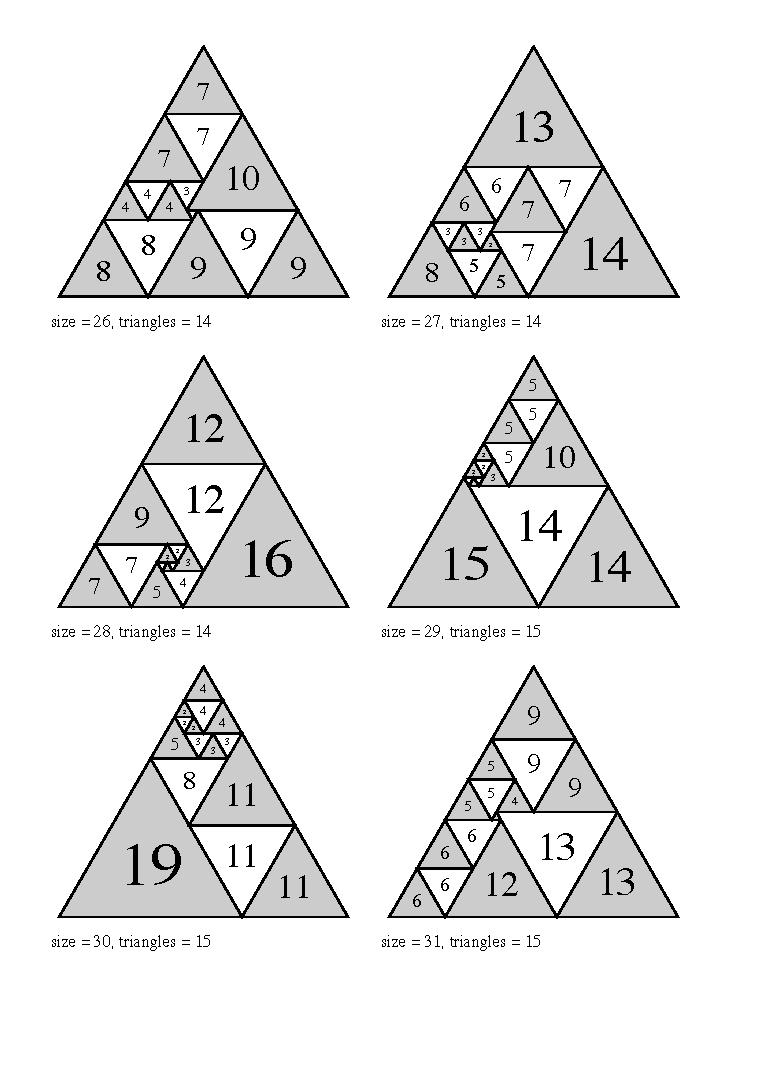
\includegraphics[trim=2em 4em 3em 2em, width=0.95\textwidth]{img/tranquility5.pdf}
\caption{Minimal triangle dissections.}
\end{figure}

\begin{figure}[htb]
\centering
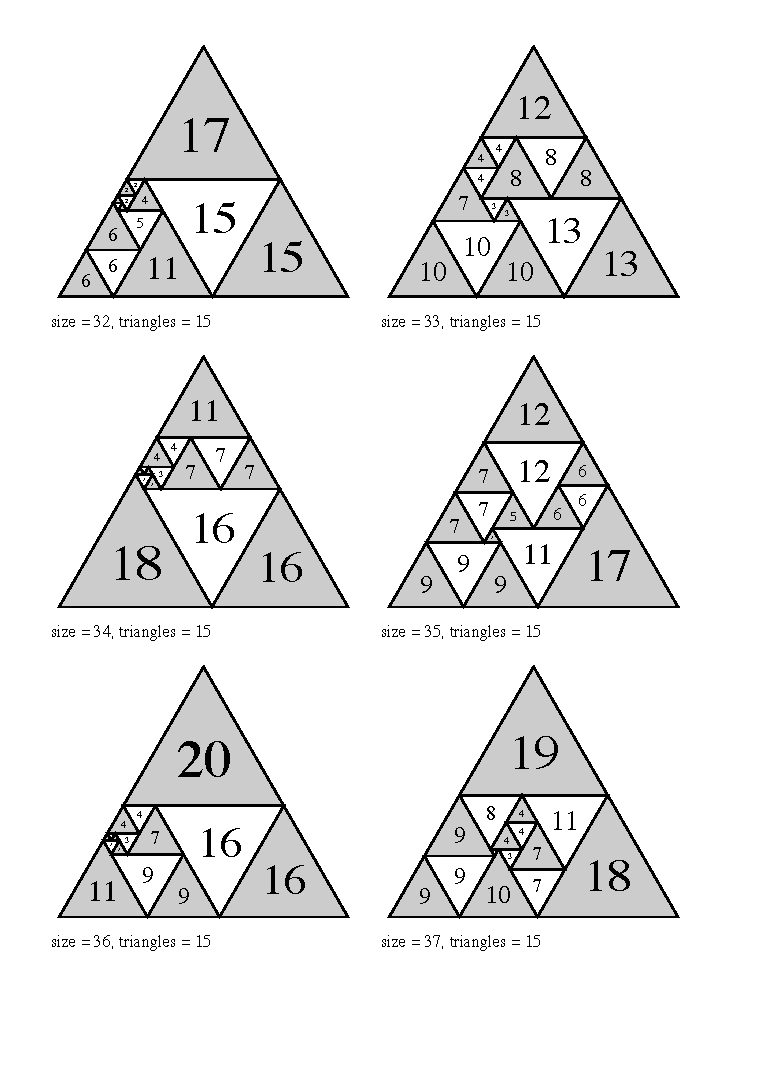
\includegraphics[trim=2em 4em 3em 2em, width=0.95\textwidth]{img/tranquility6.pdf}
\caption{Minimal triangle dissections.}
\end{figure}

